\section{Semantic Segmentation with Convolutional Neural Network}
\label{sec:network}
This section will present the convolutional neural network in detail. \todo[inline]{Better and a slightly longer introduction to section}

\subsection{Patch-based architecture}
\todo[inline]{Explain what this actually does!}
\todo[inline]{Outline what this thing actually predict. Patch based approach}
\todo[inline]{Input bigger than output. Context, etc}
\todo[inline]{Explain layering etc. show image}
\todo[inline]{Have to justify model layering. 256 output? why 64x64 input images why? Context. }

The system is based on the deep neural network outlined by \cite{Mnih_aerial_images_noisy}. The network have three convolutional layers and two fully connected layers. This network architecture is depicted in Figure \ref{fig:conv}. After the network is trained, it can predict whether or not roads are present in a $16 \times 16$ pixel area contained in the center of a $64 \times 64$ aerial image patch. The input patch is considerably larger than the output patch, so that the network can better utilize the context in the image. \\

The first layer perform convolution using $13 \times 13$ kernels, and outputs in total 64 feature maps. Only the first layer utilize max pooling, which reduces the number of inputs to the next layer as well as introducing some translational invariance to the model. The kernel size in the second and third layer are currently $4 \times 4$ and $3 \times 3$, respectably. The output of the third convolutional layer is used as input to a fully connected neural network with a single hidden layer and an output layer. The latter contains 256 units where each output is the probability of a pixel representing a road.\\

\begin{figure}
\begin{center}
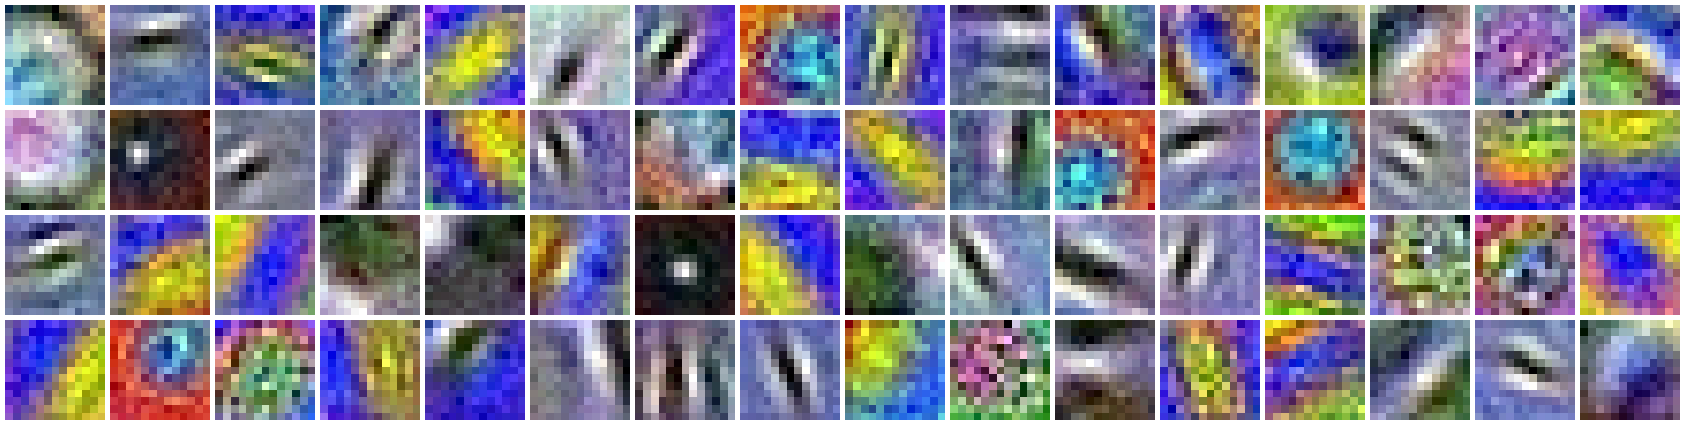
\includegraphics[width=1\columnwidth]{figs/network/Filter_unblurred.png}
\caption[Visualization of filter map]{Visualization of filter maps from the first convolutional layer of a trained network.}
\label{fig:convoluional_first_layer_visualization}
\end{center}
\end{figure}

\begin{table}[htp]
\caption{Hyperparameters for \ac{CNN}}
\begin{center}
\begin{adjustbox}{max width=\textwidth}
\begin{tabular}{+l ^l ^l}\hline
\rowstyle{\bfseries}
  Parameter & Description & Value\\\hline
  $K_i$ & Number of kernels for convolutional layer i & 64, 112, 80 \\
  $CLF_i$ & Filter size of convolutional layer $i$ & (13,13),(4,4),(3,3) \\
  $CLS_i$ & Stride amount of convolutional layer $i$ & (4,4),(1,1),(1,1) \\
  $CLP_i$ & Pool size of convolutional layer $i$ & (2,2),(1,1),(1,1) \\
  Cost function & Function that is minimzed each iteration & Cross entropy \\
  Epochs & How many epochs \ac{CNN} will train for. & 100 \\
  $\theta_i$ & Transfer function for each value & Leaky ReLU x4, sigmoid x1 \\
  $h$ & Number of neurons in hidden layer. & 4096 \\
  $p_i$ & Dropout rate for a layer $i$ & 1.0, 0.9, 0.8, 0.5, 1.0 \\
  $a$ & Learning rate & 0.0014 \\
  $a_{decrease}$ & learning rate decrease factor & 0.95 \\
  $L_2$ & Weight decay & 0.0001 \\
  $m$ & Momentum & 0.9 \\
  $b$ & Batch size & 64 \\\hline
\end{tabular}
\end{adjustbox}
\end{center}
\label{tab:curriculum_parameters}
\end{table}

\subsection{Optimization}
\todo[inline]{BETA 0.0.0.1 Really bad, explanation. But something}
%\url{http://cs231n.github.io/neural-networks-3/}
%http://www.cs.toronto.edu/~tijmen/csc321/slides/lecture_slides_lec6.pdf}
%http://arxiv.org/pdf/1212.0901v2.pdf
%http://stats.stackexchange.com/questions/179915/whats-the-difference-between-momentum-based-gradient-descent-and-nesterovs-ac
The model parameters are optimized with a special form of \ac{SGD}, called Nesterov momentum stochastic gradient decent, and have an improved stability and faster convergence compared to standard \ac{SGD} \citep{Bengio_advances_optimizing}. The standard momentum approach extend the gradient update step, by introducing velocity. The loss can be interpreted as a hilly error surface where loss optimization can be viewed as a particle gaining and losing velocity while interacting with the landscape. When the loss optimization is gaining velocity, it will stop doing steepest decent, and results in a smoother decent with less oscillations. Basically, instead of directly using the gradient to move in the landscape, the gradient will influence the velocity. The only hyperparameter associated with momentum is $m$, which damps the velocity, and can be interpreted as friction. \\


Nesterov momentum is a variation of momentum. Unlike standard momentum, the Nesterov method first makes a step in the direction of the accumulated velocity, and then makes a correction of the velocity based on the new location. In standard momentum a correction to the velocity is made before taking a step. The Nesterov gradient is defined by the following update rule:

\begin{flalign*}
     &v_{t} = mv_{t-1} - a \nabla f(\theta_{t-1} + m v_{t-1}) \\
     &\theta_t = \theta_{t-1} + v_t,
\end{flalign*}

\noindent where $\theta_t$ is the model parameters, $v_t$ the velocity, $m$ the momentum decay, $a$ the current learning rate and $\nabla f(\theta)$ is the gradient.\\

Furthermore, the system also support RMSProp which keeps a running average of the gradient magnitude for every weight. This is used to adaptively adjust the learning rate of each weight. Compared to regular \ac{SGD}, this will result in a faster convergence. \todo{Paper detailing RMSprop}\\ 

All the above mentioned optimization approaches have an important hyperparameter in common, and that is the learning rate $a$. In this implementation the learning rate is annealed over time, by step decay. The learning rate is decreased in regular intervals of epochs by some factor $a_{decrease}$ during optimization. \\

\todo[inline]{Learning and negative log likelihood?. Optimization of the loss. So the loss is negative log likelihood}

\subsection{Regularization}
\todo[inline]{small introduction to what regularization can do}
\todo[inline]{Dropout}
\todo[inline]{What it is. Why it is useful. Paper. Why dropout in convolutional layers.}
\todo[inline]{Must be scaled at test time. No dropping then}

\todo[inline]{L2 regularization}
\todo[inline]{What is L2 good for?}

\todo[inline]{Early stopping}
\todo[inline]{Leaky ReLu}
\todo[inline]{Can this be placed here?}

To avoid overfitting the training data, and hopefully achieve better generalization, different regularization schemes are applied during optimization, such as L2 weight decay, early stopping, and dropout. The first applies a weight penalty to prevent weights from growing large. The second stops the optimization process when performance on the validation set starts to consistently decrease. This is an indication of the model starting to overfit the training set. Dropout forces the units to rely less on each other, by randomly disabling half of the units in the network during training. This encourage units to encode independently useful information, since dropout penalize co-adaptation between units.\\


\subsection{Data preprocessing}
\todo[inline]{Beta 0.0.0.01 Rubbish}
The datasets used in this thesis contains aerial images and road label maps that are very large. Each image is typically around $1500 \times 1500$ pixels in size, which is arguably to large for the model to training with. Smaller patches of examples are therefore extracted from these larger images. From each image a certain number of data patches and label patches of $64 \times 64$ and $16 \times 16$ are extracted randomly and added to a patch dataset.\\

However, before extracting patches, each aerial image and road label map is rotated by a random number of degrees between 0 and 360 degrees. This is necessary because of orientation bias in the datasets \todo{DO they?}. In many cities the road network is often constructed in a grid pattern, which leads to roads having certain orientations. Without random rotations of the training data, the model might become better at detecting roads only at certain orientations \citep{Mnih_roads_high_res_aerial_images}. Each image is therefore rotated by random angles before extracting patches, which results in a patch training set that encourages the model to learn invariance to orientation.\\

Another data augmentation method utilized when constructing the patch training set is flipping. This is a common method for artificially increase the size of the dataset \citep{Krizhevsky_imagenet}. Since the dataset contains aerial imagery that depict landscape from a top-down perspective, the patches can both be flipped vertically and horizontally \todo{Something missing here}.\\

Contrast normalization is also applied to every patch. each patch is normalized by subtracting the mean pixel value from the pixels of a patch, and then dividing the result by the standard deviation found for all pixels in the dataset.\\

Additionally, the datasets used exhibit some class imbalance \citep{Japkowicz_class_imbalance}, which can be problematic since the model might decide to prioritize loss minimization of the high-occurence classes and ignore low-occurring classes. Random sampling of the datasets, lead to a large imbalance between road examples and non-road examples. The proportion of patches containing road according to the labelling, range between 8\% and 25\%\todo{Check numbers}, depending on the dataset. This is solved by simply artificially increasing the proportion of road examples, when sampling the patch dataset. This method is not applied to the test and validation patch set, and will therefore retain their natural class distribution\todo{Improve language}.\\